\chapter{Implementacija i korisničko sučelje}
		
		
		\section{Korištene tehnologije i alati}
		
			%\textbf{\textit{dio 2. revizije}}
			 Komunikacija u timu realizirana je korištenjem aplikacije Discord\footnote{https://discord.com/}, a kao sustav za upravljanje izvornim kodom Git\footnote{https://git-scm.com/}. Za izradu UML dijagrama korišten je alat VisualParadigm\footnote{https://online.visual-paradigm.com/}. Udaljeni repozitorij projekta je dostupan na web platformi GitHub\footnote{https://github.com/}.
			 
			 Kao uređivač izvornog koda korišten je Visual Studio Code\footnote{https://code.visualstudio.com/} napravljen od strane Microsofta s Electron Frameworkom, za Windows, Linux i macOS. Dolazi s ugrađenom podrškom za JavaScript, TypeScript i Node.js te ima bogat ekosustav proširenja za druge jezike i runtimeove. Neke od značajki uključuju podršku za debugiranje, isticanje sintakse, inteligentno dovršavanje koda, isječke, refaktoriranje koda i ugrađeni Git.
			 
			 Za modeliranje baze podataka korišten je web alat ERDPlus\footnote{https://erdplus.com/} koji između ostalog omogućuje jednostavno stvaranje ER dijagrama i relacijskih shema. Ovaj besplatan alat pruža pomoć u vizualizaciji i efikasnom dizajniranju baza podataka pomoću automatskog generiranja SQL DDL (Data Definition Language) izjava na temelju korisnički unesenih shema.
             
			 Od sustava za upravljanje bazama podataka korišten je PostgreSQL\footnote{ https://www.postgresql.org/}. Sustav poštuje ACID principe pri izvođenju transakcija, proširljiv je i drži se većine SQL:2011 standarda.
			 
			 Aplikacija je napisana koristeći web okvir Flask\footnote{https://flask.palletsprojects.com/en/3.0.x/}. Razvijen je od strane Armina Ronachera, vođe Međunarodne grupe entuzijasta za Python. Temelji se na WSGI alatima i Jinja2 predlošku. Ovaj okvir pokriva širok spektar primjene, od osnovnih koncepta kao što su postavljanje i instalacija do naprednijih koncepta poput autentifikacije korisnika i integracije baze podataka.
			 
			 Za izradu frontenda korišten je React\footnote{https://reactjs.org/} i jezik JavaScript\footnote{https://www.javascript.com/}. React, također poznat kao React.js ili ReactJS, je biblioteka u JavaScriptu za izgradnju korisničkih sučelja. Održavana je od strane Facebooka. React se najčešće koristi kao osnova u razvoju web ili mobilnih aplikacija. Složene aplikacije u Reactu obično zahtijevaju korištenje dodatnih biblioteka za interakciju s API-jem.

			 Kao pomoć u razvoju korištena je usluga ElephantSQL\footnote{https://www.elephantsql.com/} za hosting baze podataka. ElephantSQL nudi korisnički prijateljsku i skalabilnu platformu za upravljanje PostgreSQL bazama podataka u oblaku. Pojednostavljuje proces opskrbe, upravljanja i skaliranja PostgreSQL instanci, omogućujući razvojnom timu da se usredotoči na funkcionalnost svoje aplikacije umjesto na upravljanje infrastrukturom.

			 S ciljem pojednostavljenja procesa slanja e-mailova koji je integriran unutar aplikacije, korišten je Mailjet\footnote{https://www.mailjet.com/} - cloud-based pružatelj usluga e-pošte (ESP) koji omogućuje slanje transakcijskih i marketinških e-mail kampanja. Mailjetova platforma osigurava pouzdano slanje na sigurnoj i robustnoj infrastrukturi koja se nalazi na Google Cloud Platformi, te nadzire i optimizira ključne analitike poput stopa otvaranja, stopa odbijanja i spam pogodaka.

			 Za pohranu slika korišten je Firebase Storage\footnote{https://firebase.google.com/products/storage/} - usluga koja dio platforme Firebase unutar Google Cloud Platform-a (GCP) i koja omogućuje pohranu i upravljanje medijima generiranim od strane korisnika web i mobilnih aplikacija. Kada koristimo Firebase Storage, datoteke se prenose izravno od i do klijenta. Kada korisnik prenese datoteku na Firebase Storage, generira se URL za tu datoteku. Taj URL se može zatim spremiti u bazu podataka na poslužitelju. Dakle, na poslužitelju ostaje samo poveznica na datoteku, a sama datoteka se pohranjuje u Firebase Storage. Ovo omogućuje efikasno upravljanje datotekama bez potrebe za velikom infrastrukturom na poslužitelju. Također, smanjuje se opterećenje na poslužitelju jer se prijenos datoteka obavlja izravno između klijenta i Firebase Storage-a.

			 Svoju primjenu u izradi ovog projekta pronašao je i Docker\footnote{https://www.docker.com/} - otvorena platforma za razvoj, isporuku i pokretanje aplikacija. Docker omogućuje odvajanje aplikacija od infrastrukture kako bi se softver mogao brzo isporučiti1. Docker pruža mogućnost pakiranja i pokretanja aplikacije u labavo izoliranom okruženju zvanom kontejner. Kontejneri su lagani i sadrže sve što je potrebno za pokretanje aplikacije. U kontekstu izrade web aplikacija, Docker pojednostavljuje razvoj omogućujući programerima stvaranje prijenosnih i konzistentnih okruženja aplikacija, smanjujući složenost postavljanja i održavanja razvojnih, testnih i produkcijskih okruženja. Kontejneri su odlični za kontinuiranu integraciju i kontinuiranu isporuku (CI/CD) radnih tokova.

             Kao platforma za deployment korišten je Render\footnote{https://render.com/} koji omogućuje brzo i jednostavno postavljanje web aplikacija. Podržava sve glavne jezike, besplatne certifikate, zaštitu od DDoS napada i automatsko postavljanje iz GitHuba. Također nudi i sučelje za brzo i jednostavno objavljivanje statičkog web sadržaja. Može se koristiti za postavljanje različitih vrsta aplikacija, uključujući Node.js, Express i Flask aplikacije.		 
			 
			 Za izradu dokumentacije korišten je LateX\footnote{https://www.latex-project.org/}, markup jezik koji svoju osnovnu primjenu nalazi u izradi znanstvenih publikacija. Osnovna mu je značajka da pisac koristi konvencije označavanja koje predstavljaju ugrađene naredbe za definiranje opće strukture dokumenta, stiliziranje teksta, dodavanje citata, unakrsnih referenci i sl.Tako stvorenu LaTeX datoteku obrađuje softver zvan TeX engine koji koristi ugrađene naredbe kako bi vodio i kontrolirao proces izgradnje profesionalno složenenog PDF dokumenta.
			\eject 
		
	
		\section{Ispitivanje programskog rješenja}
			
			\textbf{\textit{dio 2. revizije}}\\
			
			 \textit{U ovom poglavlju je potrebno opisati provedbu ispitivanja implementiranih funkcionalnosti na razini komponenti i na razini cijelog sustava s prikazom odabranih ispitnih slučajeva. Studenti trebaju ispitati temeljnu funkcionalnost i rubne uvjete.}
	
			
			\subsection{Ispitivanje komponenti}
			\textit{Potrebno je provesti ispitivanje jedinica (engl. unit testing) nad razredima koji implementiraju temeljne funkcionalnosti. Razraditi \textbf{minimalno 6 ispitnih slučajeva} u kojima će se ispitati redovni slučajevi, rubni uvjeti te izazivanje pogreške (engl. exception throwing). Poželjno je stvoriti i ispitni slučaj koji koristi funkcionalnosti koje nisu implementirane. Potrebno je priložiti izvorni kôd svih ispitnih slučajeva te prikaz rezultata izvođenja ispita u razvojnom okruženju (prolaz/pad ispita). }
			
			
			
			\subsection{Ispitivanje sustava}
			
			 \textit{Potrebno je provesti i opisati ispitivanje sustava koristeći radni okvir Selenium\footnote{\url{https://www.seleniumhq.org/}}. Razraditi \textbf{minimalno 4 ispitna slučaja} u kojima će se ispitati redovni slučajevi, rubni uvjeti te poziv funkcionalnosti koja nije implementirana/izaziva pogrešku kako bi se vidjelo na koji način sustav reagira kada nešto nije u potpunosti ostvareno. Ispitni slučaj se treba sastojati od ulaza (npr. korisničko ime i lozinka), očekivanog izlaza ili rezultata, koraka ispitivanja i dobivenog izlaza ili rezultata.\\ }
			 
			 \textit{Izradu ispitnih slučajeva pomoću radnog okvira Selenium moguće je provesti pomoću jednog od sljedeća dva alata:}
			 \begin{itemize}
			 	\item \textit{dodatak za preglednik \textbf{Selenium IDE} - snimanje korisnikovih akcija radi automatskog ponavljanja ispita	}
			 	\item \textit{\textbf{Selenium WebDriver} - podrška za pisanje ispita u jezicima Java, C\#, PHP koristeći posebno programsko sučelje.}
			 \end{itemize}
		 	\textit{Detalji o korištenju alata Selenium bit će prikazani na posebnom predavanju tijekom semestra.}
			
			\eject 
		
		
		\section{Dijagram razmještaja}
			
			%\textbf{\textit{dio 2. revizije}}
			
			 %\textit{Potrebno je umetnuti \textbf{specifikacijski} dijagram razmještaja i opisati ga. Moguće je umjesto specifikacijskog dijagrama razmještaja umetnuti dijagram razmještaja instanci, pod uvjetom da taj dijagram bolje opisuje neki važniji dio sustava.}
			 Sustav je baziran na arhitekturi ”klijent – poslužitelj”, a klijenti koriste web preglednik kako bi pristupili web aplikaciji. Na poslužiteljskom računalu nalaze se poslužitelj frontend dijela web aplikacije, poslužitelj backend dijela web aplikacije te poslužitelj baze podataka. Backend dio aplikacije nalazi se unutar Docker kontejenera koji predstavlja okruženje koje sadrži sve što je potrebno za izvođenje dotičnog dijela aplikacije. Pohrana slika realizirana je uz pomoć usluge Firebase Storage koja je dio Firebase-a, platforme za razvoj mobilnih i web aplikacija. Firebase Storage se za pohranu i dohvat korisnički generiranih sadržaja oslanja na uslugu Google Cloud Storage. Sve spomenute usluge dio su šire platforme pod nazivom Google Cloud Platform (GCP). Odgovornost backend dijela web aplikacije je da prihvati generiranu javnu poveznicu na tu sliku i pohrani je u bazu podataka nakon što se korisnička slika otpremi na Firebase Storage. Firebase Storage omogućuje izravan prijenos datoteka od i do klijenta čime se rasterećuje poslužitelj koji samo procesuira poveznice. Komunikacija između osnovnih dijelova sustava odvija se preko HTTPS veze.
			 \begin{figure}[htbp]
				\centering
				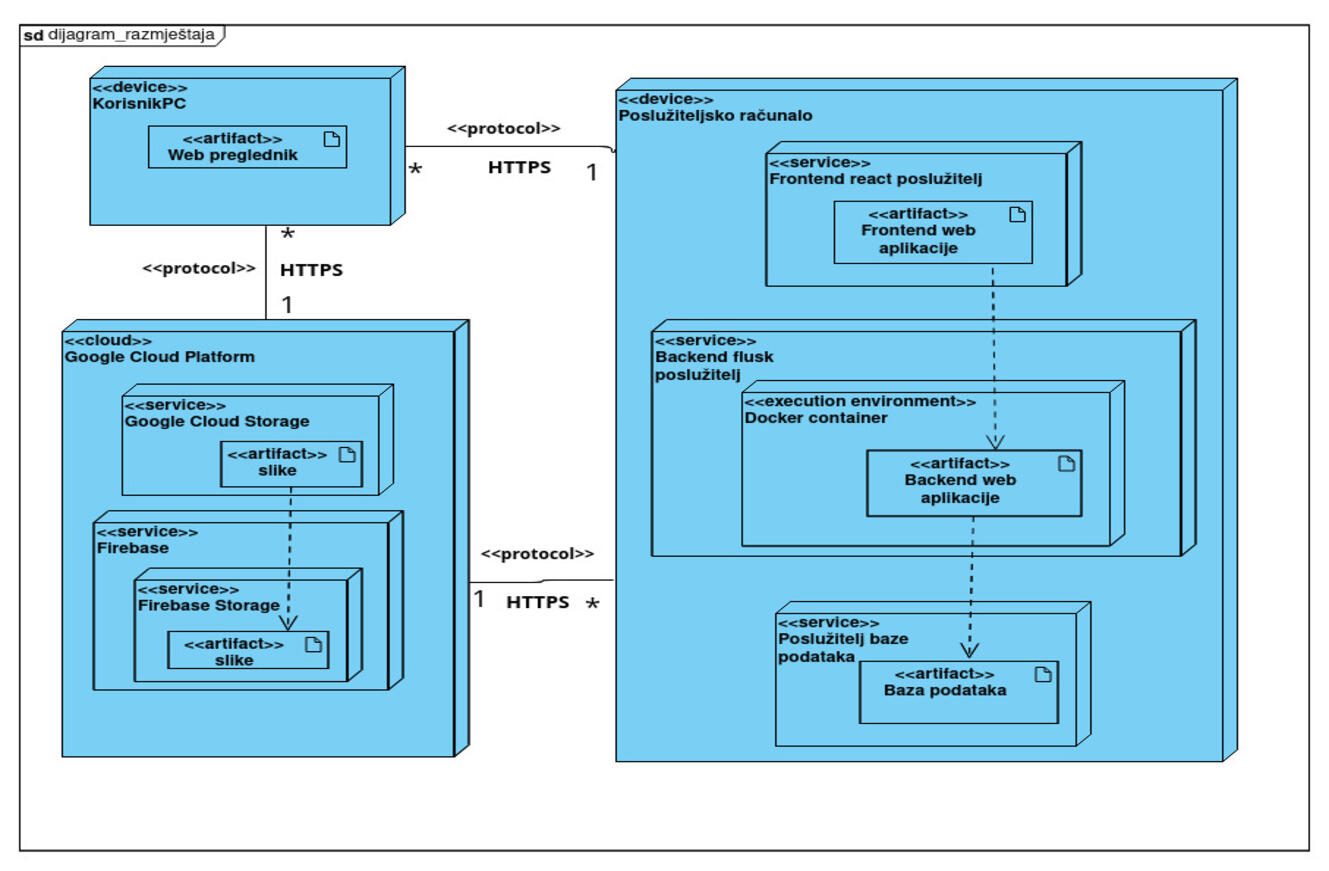
\includegraphics[width=1\textwidth]{dijagrami/diagram_razmjestaja_new2.jpeg}
				\caption{Dijagram razmještaja}
			\label{fig:my_image}
			\end{figure}
			\eject 
		
		\section{Upute za puštanje u pogon}
		
			\textbf{\textit{dio 2. revizije}}\\
		
			 \textit{U ovom poglavlju potrebno je dati upute za puštanje u pogon (engl. deployment) ostvarene aplikacije. Na primjer, za web aplikacije, opisati postupak kojim se od izvornog kôda dolazi do potpuno postavljene baze podataka i poslužitelja koji odgovara na upite korisnika. Za mobilnu aplikaciju, postupak kojim se aplikacija izgradi, te postavi na neku od trgovina. Za stolnu (engl. desktop) aplikaciju, postupak kojim se aplikacija instalira na računalo. Ukoliko mobilne i stolne aplikacije komuniciraju s poslužiteljem i/ili bazom podataka, opisati i postupak njihovog postavljanja. Pri izradi uputa preporučuje se \textbf{naglasiti korake instalacije uporabom natuknica} te koristiti što je više moguće \textbf{slike ekrana} (engl. screenshots) kako bi upute bile jasne i jednostavne za slijediti.}
			
			
			 \textit{Dovršenu aplikaciju potrebno je pokrenuti na javno dostupnom poslužitelju. Studentima se preporuča korištenje neke od sljedećih besplatnih usluga: \href{https://aws.amazon.com/}{Amazon AWS}, \href{https://azure.microsoft.com/en-us/}{Microsoft Azure} ili \href{https://www.heroku.com/}{Heroku}. Mobilne aplikacije trebaju biti objavljene na F-Droid, Google Play ili Amazon App trgovini.}
			
			
			\eject 